% === VI. Analisis Kebutuhan dan Desain Solusi Perangkat Lunak ===
\secbox{VI.}{Analisis Kebutuhan dan Desain Solusi Perangkat Lunak}

\subsecbar{6.1 Analisis Kebutuhan}
Berdasarkan hasil identifikasi kebutuhan pengguna dan studi literatur, kebutuhan perangkat lunak LUNA dibagi menjadi dua kategori, yaitu kebutuhan fungsional dan kebutuhan nonfungsional.

\subsubsecstyle{1. Kebutuhan fungsional}
\begin{enumerate}[leftmargin=*,label=\alph*.]
    \item Menyediakan dialog empatik yang terpersonalisasi sesuai profil dan kondisi emosional pengguna.
    \item Menghasilkan \textit{Automatic Diary Generation} dari hasil percakapan.
    \item Mengelola \textit{Long-term Conversation Memory} untuk menyimpan dan memanggil kembali informasi penting pengguna.
    \item Melakukan analisis emosi dan sentimen secara \textit{real-time}.
    \item Mendeteksi krisis emosional serta mengaktifkan protokol penanganan dan rekomendasi bantuan darurat.
    \item Memberikan rekomendasi latihan relaksasi, teknik CBT mandiri, dan materi psikoedukasi berbasis bukti klinis.
    \item Mendukung komunikasi suara melalui \textit{Speech-to-Text} dan \textit{Text-to-Speech}.
\end{enumerate}

\subsubsecstyle{2. Kebutuhan nonfungsional}
\begin{enumerate}[leftmargin=*,label=\alph*.]
    \item Menjamin keamanan data melalui enkripsi dan anonimisasi informasi pribadi.
    \item Menggunakan \textit{Retrieval-Augmented Generation} (RAG) berbasis literatur klinis untuk meningkatkan akurasi respons dan meminimalkan halusinasi.
    \item Menyediakan waktu respons yang cepat untuk percakapan teks maupun suara secara \textit{real-time}.
    \item Menyajikan antarmuka yang intuitif, nyaman, dan mudah digunakan oleh Generasi Z.
\end{enumerate}

\subsecbar{6.2 Desain Solusi}
Desain solusi LUNA disusun untuk menggambarkan konsep, arsitektur, dan mekanisme kerja sistem dalam mewujudkan layanan pendamping kesehatan mental berbasis Multi-Agent Artificial Intelligence. Bagian ini menjelaskan rancangan solusi yang menjadi dasar pengembangan perangkat lunak secara terstruktur.

\subsubsecstyle{1. Gambaran solusi}
\begin{figure}[H]
    \centering
    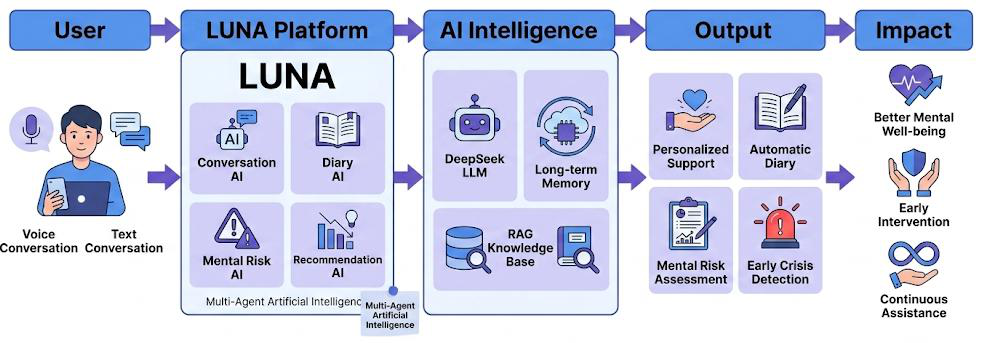
\includegraphics[width=0.80\textwidth]{images/bab6/fig3_konsep.png}
    \caption{Gambaran Konsep LUNA}
\end{figure}

\subsubsecstyle{2. Kerangka Evaluasi Risiko \& Integrasi DASS-21}
Dalam mengevaluasi kondisi emosional pengguna, LUNA mengintegrasikan instrumen psikometris \textbf{DASS-21 (\textit{Depression Anxiety Stress Scale 21})} yang divalidasi oleh pakar psikologi. DASS-21 mengevaluasi tiga subskala emosional utama:
\begin{enumerate}[leftmargin=*,label=\arabic*.]
    \item \textbf{Subskala Depresi}: Mengukur tingkat keputusasaan, devaluasi diri, dan hilangnya minat (7 butir pertanyaan).
    \item \textbf{Subskala Kecemasan (\textit{Anxiety})}: Mengukur respons gairah otonom, efek fisiologis, dan kecemasan situasional (7 butir pertanyaan).
    \item \textbf{Subskala Stres}: Mengukur ketegangan persisten, iritabilitas, dan kesulitan bersantai (7 butir pertanyaan).
\end{enumerate}

Perhitungan skor pada masing-masing subskala dilakukan dengan menjumlahkan nilai butir (skala 0--3) lalu dikalikan 2 ($\mathrm{Skor} = \mathrm{Total\ Subskala} \times 2$). Berdasarkan norma psikometris DASS-21, skor tersebut dikelompokkan ke dalam tiga tingkatan level distres emosional:
\begin{itemize}[leftmargin=*]
    \item \textbf{Level 1 (Tingkat Ringan / \textit{Mild})}: Pengguna mengalami distres emosional ringan. LUNA memberikan psikoedukasi, validasi emosi, dan latihan relaksasi mandiri.
    \item \textbf{Level 2 (Tingkat Sedang / \textit{Moderate})}: Pengguna mengalami distres emosional sedang. LUNA mengaktifkan pendampingan CBT interaktif, penelusuran diari emosional, dan rekomendasi aktivitas terstruktur.
    \item \textbf{Level 3 (Tingkat Berat / \textit{Severe} -- \textit{Extremely Severe})}: Pengguna mengalami distres emosional tinggi atau indikasi krisis. Sistem \textit{RiskAssessmentService} secara otomatis memicu protokol \textit{Safety Gate} untuk memberikan modul bantuan darurat dan rujukan ke kontak profesional/hotline.
\end{itemize}

Hasil penilaian DASS-21 diteruskan ke komponen backend \textit{RiskAssessmentService} untuk menentukan strategi pendampingan yang tepat tanpa melakukan diagnosis medis formal.

\clearpage
\subsubsecstyle{3. Arsitektur sistem}
\begin{figure}[H]
    \centering
    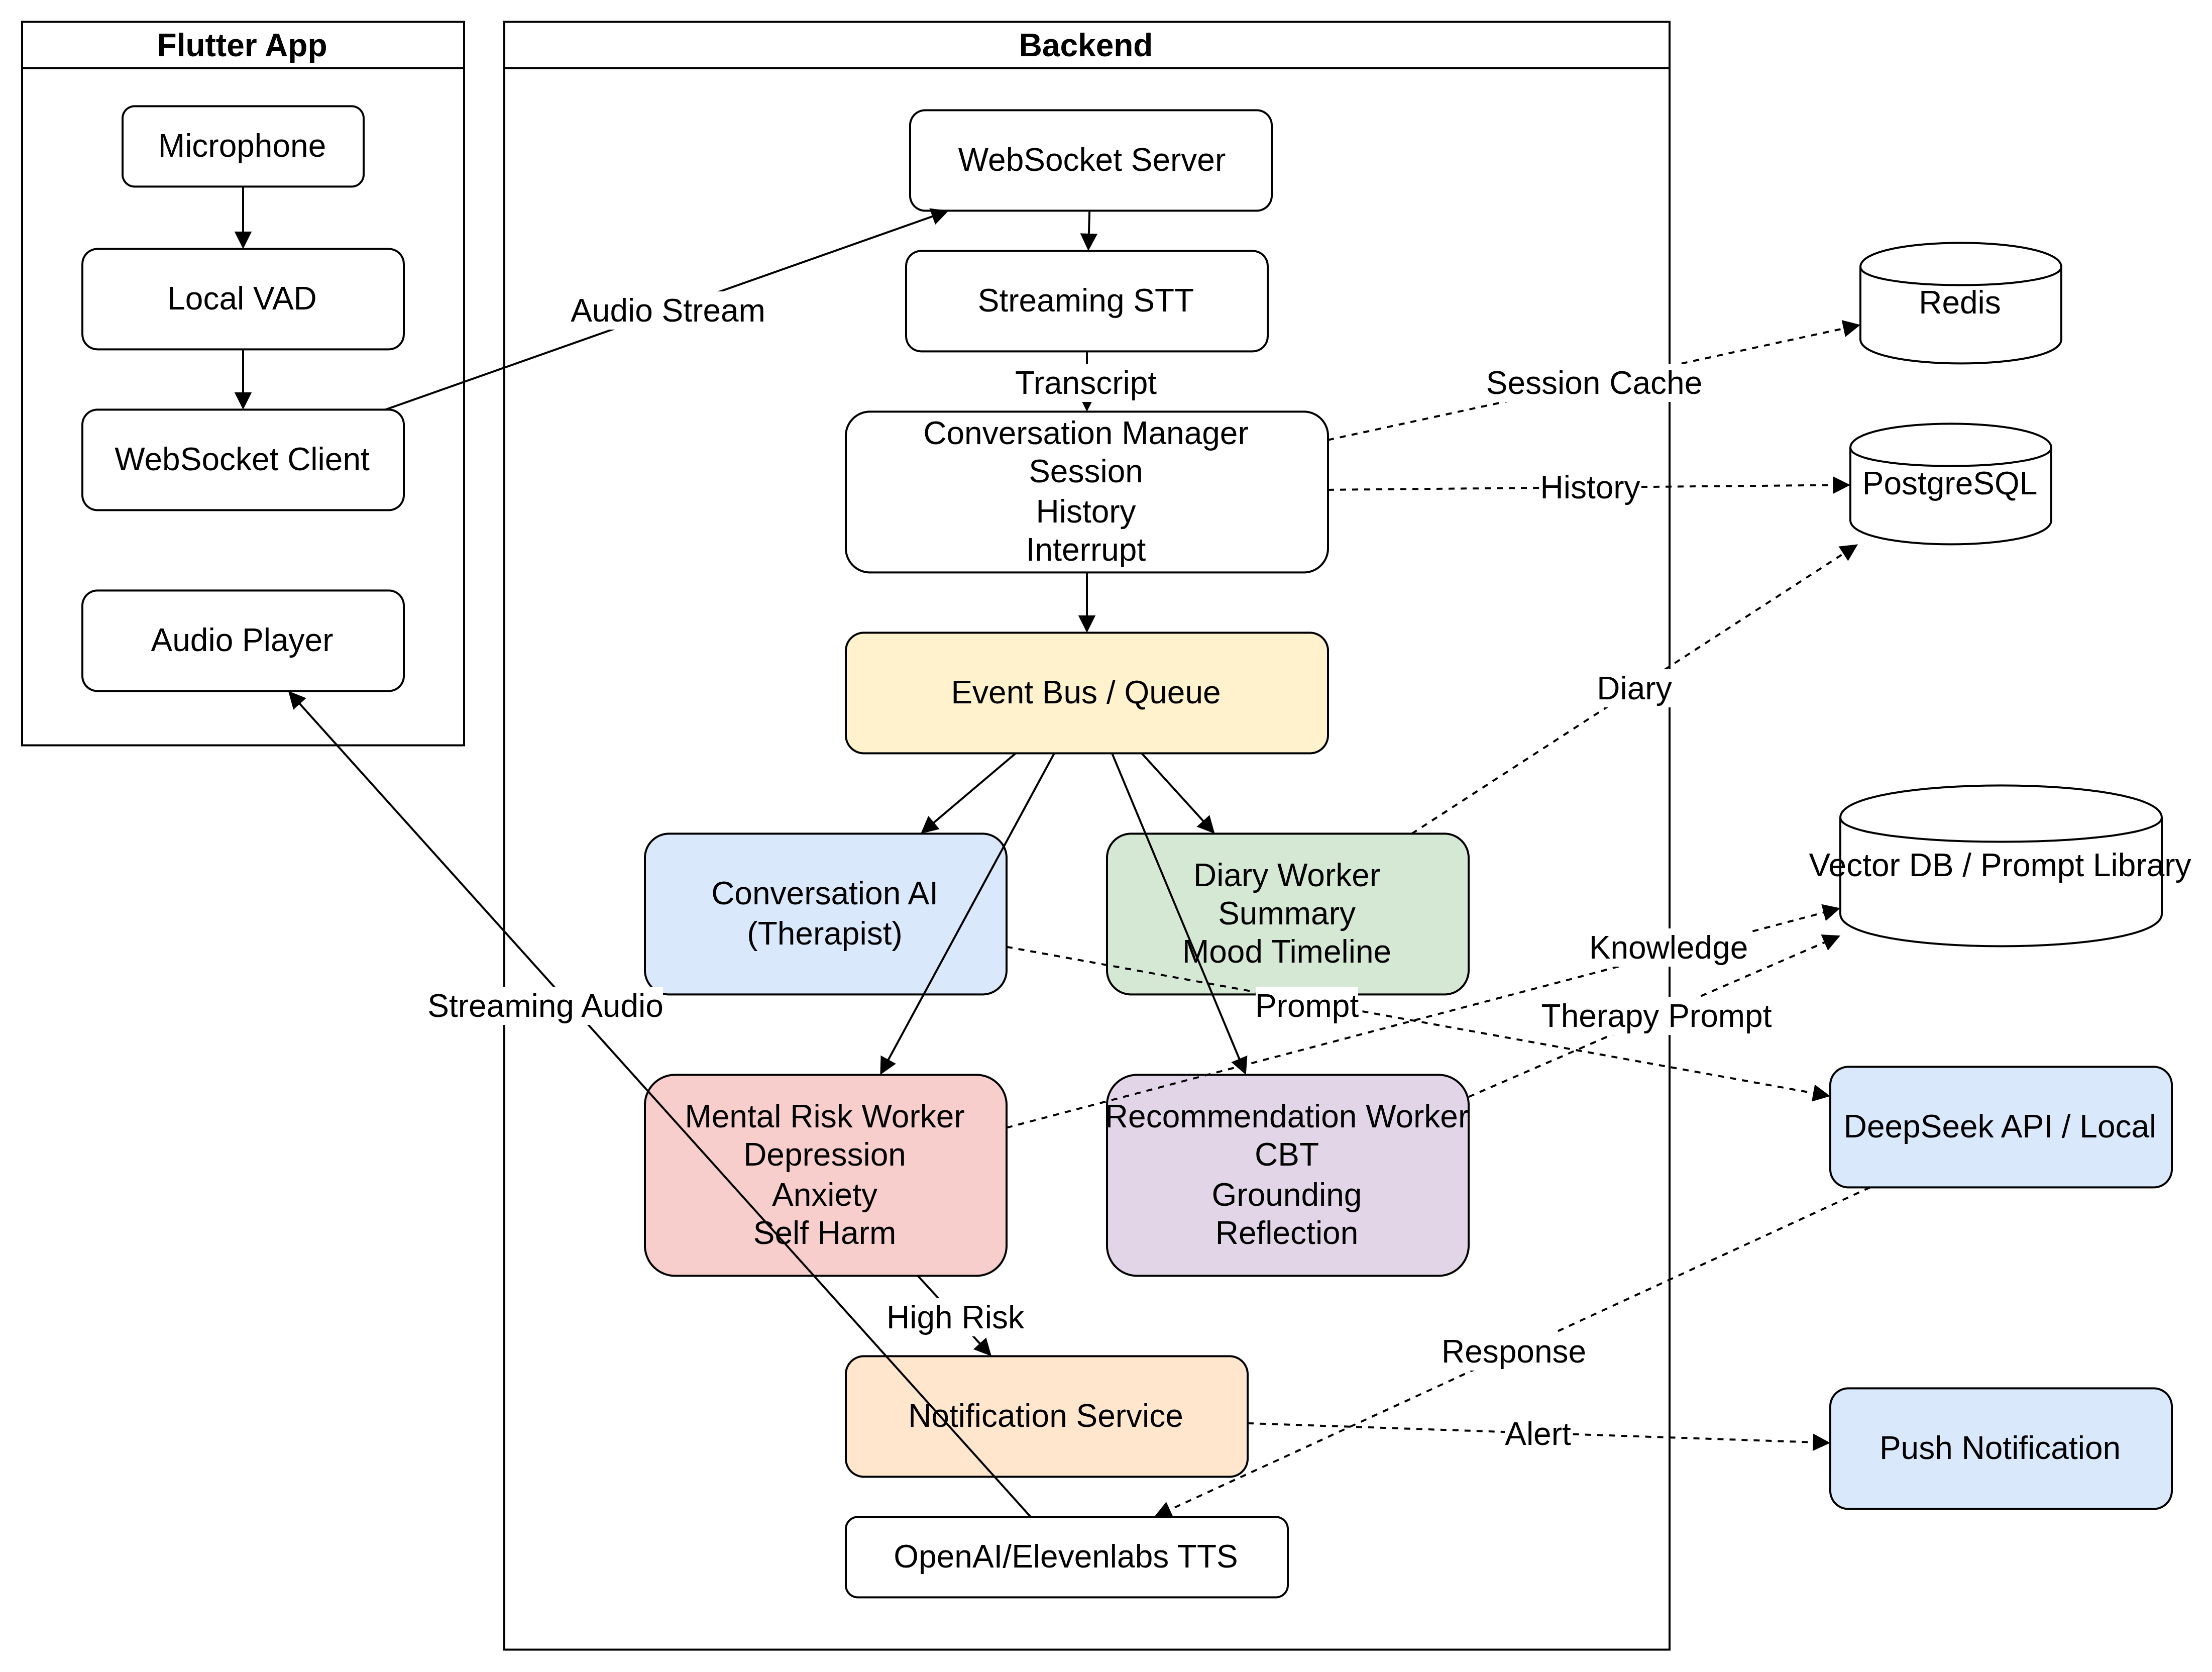
\includegraphics[width=0.85\textwidth]{images/bab6/fig4_arsitektur.png}
    \caption{Arsitektur LUNA}
\end{figure}
